\documentclass[11pt,a4paper]{article}
% Shared preamble for RuPhO English problem statements (match T1 2026 style).
% Use: \input{latex/rupho_en_preamble.tex} after \documentclass.
\usepackage[margin=1in]{geometry}
\usepackage{amsmath,amssymb}
\usepackage{graphicx}
\usepackage{float}
\usepackage{enumitem}
\usepackage{microtype}
\usepackage{caption}
\usepackage{tabularx}
\usepackage{hyperref}

\captionsetup{font=small,labelfont=bf,skip=6pt}

\setlist[itemize]{leftmargin=1.2cm}
\setlist[enumerate]{leftmargin=1.2cm}

% One outer box per subproblem: [id | statement | points] (no inner rules)
\newcommand{\problembox}[3]{%
  \par\addvspace{0.42em}%
  \noindent
  \setlength{\fboxsep}{7.5pt}%
  \setlength{\fboxrule}{0.95pt}%
  \fbox{%
    \begin{minipage}{\dimexpr\linewidth-2\fboxsep-2\fboxrule\relax}
    \begin{tabularx}{\linewidth}{@{}>{\raggedright\arraybackslash\bfseries}p{2.1em} @{\hspace{0.9em}} >{\raggedright\arraybackslash}X @{\hspace{0.9em}} >{\raggedleft\arraybackslash\bfseries}p{2.4em}@{}}
    #1 & #2 & #3
    \end{tabularx}
    \end{minipage}%
  }%
  \par\addvspace{0.32em}%
}


\title{\textbf{Bacteriorhodopsin research}}
\author{\normalsize X16 (2016) --- English translation}
\date{}
\begin{document}
\maketitle

In this task we will touch upon the issues of studying photoactive membrane proteins. These studies took place at the dawn of biophysics, in the 1970s and 80s. Wherever in this problem you need to make numerical estimates, you can use the data from the graphs and diagrams given in the condition, as well as the results of calculations from the previous paragraphs of the problem. First, let's consider a model of a cell membrane---a lipid bilayer. The lipid molecule consists of a polar head and hydrophobic tails (fatty acid residues) (Fig.~1). If you try to dissolve lipid molecules in water (a polar solvent), they can form various structures that minimize the energy of the system. That is, the polar heads of the molecules tend to form contacts with water, and the hydrophobic tails tend to hide from water.

Fig.~1. Lipid molecule

\begin{figure}[H]
    \centering
    
\includegraphics[width=0.72\textwidth]{T1_EN_assets/fig1.jpg}
    \caption{Figure 1.}
\end{figure}

The lipid bilayer is a thin polar membrane consisting of two layers of lipid (Fig.~2). This bilayer, which makes up the cell membrane, allows various ions, proteins and other molecules to be retained in the cell.

Fig.~2. Lipid bilayer

\begin{figure}[H]
    \centering
    
\includegraphics[width=0.72\textwidth]{T1_EN_assets/fig2.jpg}
    \caption{Figure 2.}
\end{figure}

For a living cell to exist, it must somehow produce energy within itself. For example, a cell can absorb sugar molecules, break them down and, using molecular mechanisms, store energy in the form of ATP (Adenosine triphosphate is a universal source of energy for all biochemical processes occurring in living systems. ATP is the main carrier of energy in the cell.). But what to do if nutrition with sugars is not available? In a study of bacteria living in extremely saline bodies of water (20\% salt), a membrane protein, bacteriorhodopsin, was discovered (Fig.~3).

Fig.~3. Bacteriorhodopsin molecule

\begin{figure}[H]
    \centering
    
\includegraphics[width=0.72\textwidth]{T1_EN_assets/fig3.jpg}
    \caption{Figure 3.}
\end{figure}

Bacteriorhodopsin turned out to be a photoactive proton pump. When a protein absorbs a photon, it transfers one proton from inside the cell to the outside. With the constant work of the protein on the cell membrane, an additional potential difference is created, which the bacterium can convert into energy and store it in the form of ATP for its needs. If these bacteria are mechanically destroyed, then flat pieces of membranes containing large quantities of bacteriorhodopsin can be isolated. This is seen as an alternative to solar panels powered by semiconductor elements. Bacteriorhodopsin, having absorbed a photon, passes through a number of intermediate states (performs a photocycle, Fig.~4). First, it throws out the proton $\rm H^+$ (L - state), which is inside the protein, and then it is replaced by the proton $\rm H^+$ from inside the cell (M - state). And until the protein returns to the ground state, it cannot absorb a new photon. The diagram shows the intermediate states in letters, as well as the characteristic transition times between them.

Fig.~4. Bacteriorhodopsin photocycle

\begin{figure}[H]
    \centering
    
\includegraphics[width=0.72\textwidth]{T1_EN_assets/fig4.jpg}
    \caption{Figure 4.}
\end{figure}

\problembox{A1}{Let flat pieces of membranes containing bacteriorhodopsin be illuminated with sufficiently powerful light. What current $I_{bR}$ flows through $1~\text{mm}^2$ of such membranes (in $\mu\text{A}/\text{mm}^2$)? From studying these membranes using electron microscopy, it is known that the density of protein molecules in them is $9\cdot{10^{12}~\text{cm}^{-2}}$}{0.50}

Various model membranes are used to functionally study various protein ion pumps. The black lipid membrane (BLM) is one such model system (Fig.~5). The experimental setup consists of two separate tanks with a highly conductive solution. A small hole with an area of $S_m=1~\text{mm}^2$ is made between the tanks. A lipid bilayer is placed over this hole. Electrodes are placed in both reservoirs, which are connected to each other through an ammeter and, in some cases, a source. A lipid membrane has electrical characteristics: capacitance $C_m$ and conductivity $G_m(=1/R_m)$, where $R_m$ is the membrane resistance. It is up to you to identify them. If the source supplies a periodic rectangular signal, then the ammeter registers a damped signal (Fig.~6). If another source supplies a periodic signal of a triangular shape, then the ammeter registers an almost rectangular signal (Fig.~7). The ammeter can be considered ideal.

Fig.~5. Diagram of a setup containing a black lipid membrane

\begin{figure}[H]
    \centering
    
\includegraphics[width=0.72\textwidth]{T1_EN_assets/fig5.jpg}
    \caption{Figure 5.}
\end{figure}

Fig.~6. Square wave $U$ and ammeter signal $I$

\begin{figure}[H]
    \centering
    
\includegraphics[width=0.72\textwidth]{T1_EN_assets/fig6.jpg}
    \caption{Figure 6.}
\end{figure}

Fig.~7. Triangle signal $U$ and ammeter signal $I$

\begin{figure}[H]
    \centering
    
\includegraphics[width=0.72\textwidth]{T1_EN_assets/fig7.jpg}
    \caption{Figure 7.}
\end{figure}

\problembox{B1}{Draw a simple equivalent electrical circuit of the membrane that describes the results well. Draw the equivalent electrical circuit for the experiment described above.}{0.50}

\problembox{B2}{Using Fig.~6 and Fig.~7, estimate the capacitance $C_m$ of the membrane. Explain your solution using formulas, graphs and diagrams}{1.00}

\problembox{B3}{Using Fig.~6 and Fig.~7, estimate the conductivity $G_m$ of the membrane. Use formulas, graphs, and diagrams to explain your solution.}{0.50}

To quantitatively characterize proton pumping by the protein, membranes containing bacteriorhodopsin are attached to a black lipid membrane (Fig.~8). Membranes with protein can attach to the black membrane in any direction; probably half of the membranes would pump protons towards the black membrane, and the other half away from the membrane. Thus, we would not be able to see any effect of the protein creating a current. To prevent this from happening, charged molecules are added to the lipids of the black membrane, which force the part of the membrane with the protein to orient itself in a preferential manner. In further calculations, assume that membranes with bacteriorhodopsin are attached to the entire surface of the black membrane (on one side).

Fig.~8. Installation diagram: membranes with protein attached to a black membrane

\begin{figure}[H]
    \centering
    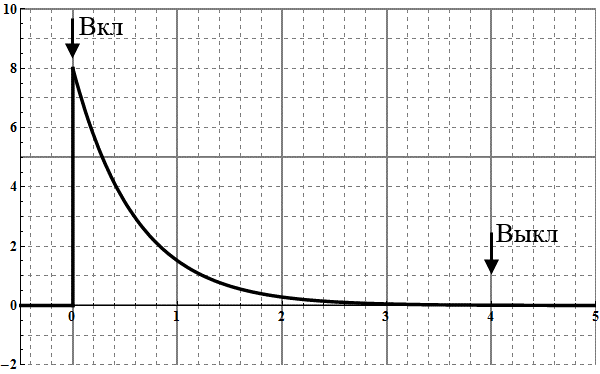
\includegraphics[width=0.72\textwidth]{T1_EN_assets/fig8.jpg}
    \caption{Figure 8.}
\end{figure}

\problembox{C1}{Let the described system of membranes be illuminated with sufficiently powerful light, such that the total current created by all proteins is constant and equal to $I_p$, and a current $I$ flows through the ammeter. Draw the equivalent electrical circuit for such an experiment.}{0.50}

\problembox{C2}{Derive a theoretical expression for the photocurrent $I(t)$ measured by an ammeter as a function of time. Express your answer in terms of the total current of proteins $I_p$, the electrical characteristics of the membrane with the protein $C_p$ and $G_p$ and the electrical characteristics of the black lipid membrane $C_m$ and $G_m$. Start the countdown $t=0$ at the moment the light is turned on.}{2.00}

In the direct experiment described above, the measured time dependence of the photocurrent turned out to be as shown in Fig.~9. The figure shows the times when the light is turned on and off. Analyzing Fig.~9, you must use the result of item $\mathrm C2$. If we conduct an experiment similar to part B of this problem, then the ratio of the capacitances of the membranes with bacteriorhodopsin and the solid membranes used to prepare the black membrane will be $C_p/C_m\approx 5$.

\begin{figure}[H]
    \centering
    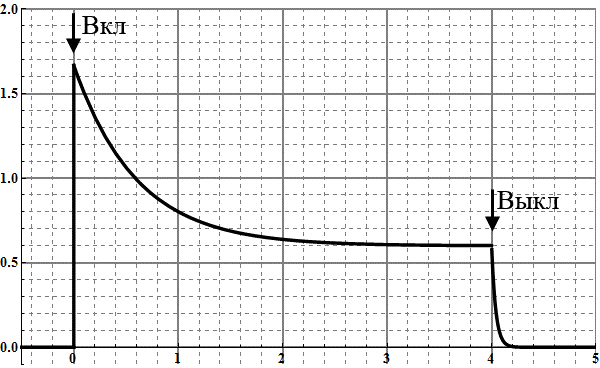
\includegraphics[width=0.72\textwidth]{T1_EN_assets/fig9.jpg}
    \caption{Figure 9.}
\end{figure}

\problembox{C3}{Using Fig.~9 and the numerical data obtained earlier, estimate the conductivity $G_p$ of membranes with protein. Use formulas, graphs, and diagrams to explain your solution.}{0.50}

\problembox{C4}{Calculate the ratio of the conductivity of the black lipid membrane and membranes with protein, i.e. find $G_m/G_p$.}{0.20}

\problembox{C5}{Using Fig.~9 and the numerical data obtained earlier, estimate the total current $I_p$ created by the proteins. Use formulas, graphs, and diagrams to explain your solution.}{0.50}

\problembox{C6}{Calculate what fraction of membranes $\alpha$ was predominantly oriented on the black membrane. Find the ratio of the number of proteins pumping protons to the membrane to their total number.}{0.30}

To study the saturability of the current generated by the proteins, the time dependence of the photocurrent was measured with varying intensity of the incident light. At low intensities, we can assume that the current created by the proteins $I_p$ is proportional to the intensity of the incident light.

Fig.~10. Dependence of the current flowing through the ammeter on time with varying intensity of incident light

\begin{figure}[H]
    \centering
    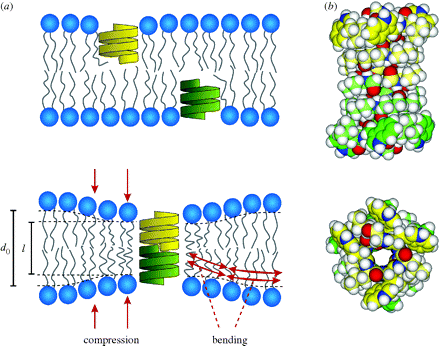
\includegraphics[width=0.72\textwidth]{T1_EN_assets/fig10_partd.png}
    \caption{Figure 10.}
\end{figure}

\problembox{D1}{Using the result of step $\mathrm C4$, making the necessary neglects, draw the equivalent electrical circuit of the experiment.}{0.20}

\problembox{D2}{Obtain an expression for the current created by the proteins, $I_p (t)$, assuming that the photocurrent $I(t)$ measured by the ammeter is known. Express your answer in terms of photocurrent $I(t)$ and the electrical characteristics of the membranes with protein and the black membrane. Start the countdown $t=0$ at the moment the light is turned on.}{1.00}

\problembox{D3}{Using the result from point $\mathrm D2$ and Fig.~10, numerically plot the graph of current $I_p$ versus time $t$. Up to the proportionality coefficient, this will be a graph of the intensity of the incident light versus time}{1.30}

It turns out that the conductivity of the black membrane can be changed using, for example, a bactericidal antibiotic, gramicidin $A$. When these molecules enter the membrane, they form a pore in the membrane (Fig.~11) through which sodium and potassium ions, as well as protons, can pass. Adding these molecules to the membrane increased its conductivity to $G^{GR}_m=10^{-8}~\Omega^{-1}$.

Fig.~11. Model of the gramicidin A molecule

\begin{figure}[H]
    \centering
    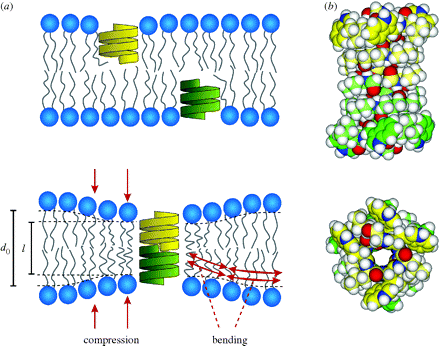
\includegraphics[width=0.72\textwidth]{T1_EN_assets/fig10.png}
    \caption{Figure 11.}
\end{figure}

\problembox{E1}{Under the experimental conditions from part $\mathrm C$ of this problem, but with increased conductivity of the black lipid membrane, redraw Fig.~9. That is, schematically depict the dependence of the photocurrent $I^{GR}(t)$ on time $t$, assuming that the fraction of membranes with protein that are predominantly oriented remains the same, and the power of the incident light is sufficient for all proteins to pump protons.}{1.00}

\vspace{1em}
\noindent\textit{Source:} \url{https://pho.rs/p/299}

\end{document}